\section{Example Line Following Robot with Deployed System and RabbitMQ - IN PROGRESS}\label{sec:example-lfr}
The example in this section concerns a line following robot (LFR). An overview
of the example is presented in \cref{fig:lfr-example-overview}.

The deployed LFR publishes its sensor readings and actuator values to RabbitMQ
Node Queue 1. However, the deployed LFR is unaware of its position on the
track and the time. For this reason, a camera is used along with image recognition to detects its position. The
Log-Translator correlates the data from the deployed LFR and the
detection before publishing it to RabbitMQ Node Queue 2. As RabbitMQ FMU subscribes
to RabbitMQ Node Queue 2 it receives the messages. The
Controller FMU and the Physical FMU make up the models of the LFR, and the
modelled LFR is aware of its position on the track.

Thus, it is possible to realise the digital twin of the deployed LFR.


\textbf{The example including a docker-compose file for
  starting a local RabbitMQ Node is IN PROGRESS and you can follow it at
  \url{https://github.com/INTO-CPS-Association/example-DT-line_following_robot}.\\
See Issues in the repository for future work on the example.}
\begin{figure}[!htb]
  \centering
  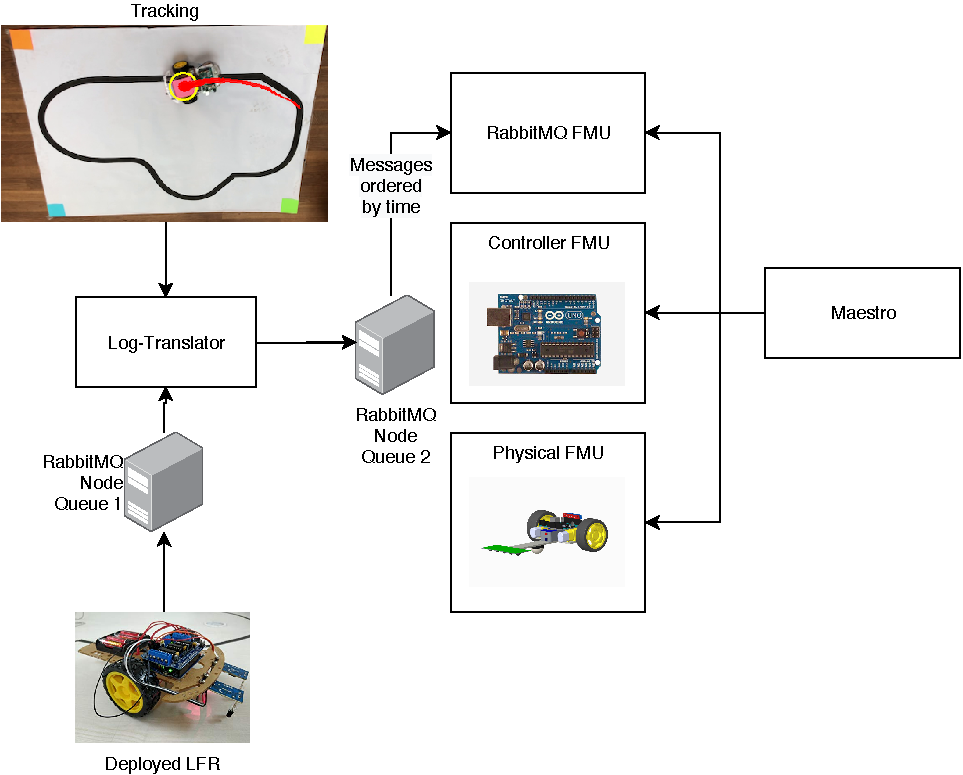
\includegraphics[width=\textwidth]{figures/lfr-example-overview.pdf}
  \caption{Water Tank}
  \label{fig:lfr-example-overview}
\end{figure}


%%% Local Variables:
%%% mode: latex
%%% TeX-master: "../rabbitmq-fmu"
%%% End:
